\documentclass[12pt]{article}
\usepackage{tikz}
\usetikzlibrary{shapes,snakes}
\usepackage{algorithm}
\usepackage{algorithmic}%\usepackage[pagebackref=true,colorlinks,linkcolor=blue,citecolor=magenta]{hyperref}
\usepackage{graphicx} 
\usepackage{fancybox}
\usepackage{setspace}  
\usepackage[colorlinks,linkcolor=blue,citecolor=magenta]{hyperref}
\usepackage{enumerate} 
%\usepackage{auto-pst-pdf} 
\usepackage{amsthm,amssymb,amsmath}
\usepackage{indentfirst}
\usepackage{listings}
\begin{document}

\title{Initial Value Computations}
\author{}
\date{}
\maketitle
%In the following sections the domain of 
\section{Graph representation of maps}
Input variables of each map can be represented in unions and or intersections of relations's variables. We can model these dependencies with a directed graph. We construct a graph $G=<V,E>$ as follow. $V$ is the union of all variables(including the bigsum variables) and the set of all maps. The set of edges consist of all directed edges of form $(a,b)$ which shows that there is an directed edge between node $a$ and $b$. Here $a$ can be a variable and/or a map name, but $b$ definitely is a map name because any variable is an independent entity which does not depend on any map or other variables. When there is $(a,b)$ edge it means that the computation of map $b$ needs the value of variable/map of $b$. 

\begin{figure}[htbp]
\begin{center}
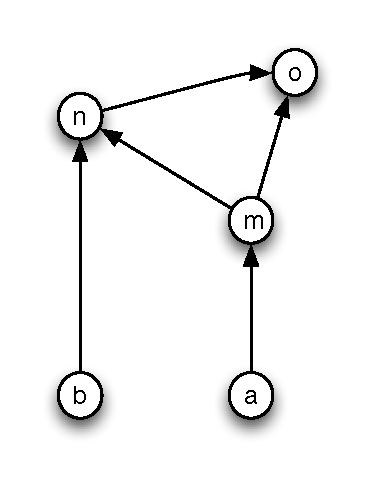
\includegraphics[scale=0.8]{fig1.eps}
\caption{Sample dependencies, $a,b$ are variables and $m,n,o$ are map names}
\label{fig1}
\end{center}
\end{figure}

Obviously this graph does not have any directed cycle. For each variable node we can have a list of pertaining relations in which that variable has occurred in the schema. With this kind of data structure we know when to alter the domain of each maps. When an new item is added to a relation we know which variables depend on the relation and we can change the domain of each map in a breadth first search(BFS).  \\

When we add/delete any value from the domain of any variable we need to propagate this modification through the dependency graph. We do this task by a layer by layer manner. Suppose we have altered variable $a$. First we change the domains of its immediate adjacent. If their domains changed we do this for the next layer and so on. When none of the adjacent of a node changed, we are not required to check the modifications to the variables' domain, since it won't change(i.e. in figure \ref{fig1} if none of $m_{1},m_{2}$ changes we don't need to check the modification of $m_{3}$).\\

When the input variable of all maps were single value, the graph would be a tree, otherwise it is a directed acyclic graph. Since each edge is considered just one time, the worst case of updating time for all domains is $O(|E|)$. 

\section{Optimizations}
There are some cases which need to compute all the domains for an insertion into a relation. For this we can reduce the Circuit Value Problem(CVP) to it. In CVP we are given a circuit and the value of the input to it, we want to compute the result of the circuit. Here we can suppose that the circuit is the query and the input values are the tuples in the database. If we consider the circuit in CNF, each clause is a map. If we add any value to the database we need to update the domain of each map if this value makes all of them non-null. \\

Although in the worst case we need to evaluate the queries to find out if a certain value is in the domain for all maps but we want to do our best to escape from these evaluations. For example when we have this rule: $0=a$ we can deduce that the domain is $a$ when domain of $a$ contains $a$ otherwise it is NULL. In this section we want to talk about these rules.

We have these production rules for all AGCA expressions:
\begin{equation*}
q::= q*q\,|\,q+q\,|\,0\,\theta q\,|\,M[][]|\,\text{const}
\end{equation*}
 
When we have $t:a\,\theta\,\text{const}$ we can simply find the domain of $t$. But when we have $a\,\theta\,T(a)$ we need to evaluate this query for all $a$ to find out its domain. 

When we have a map which non of its sub maps' domains have changed we don't need to compute the domain for any modifications, it won't change. 

\end{document}
